\section{\cjdt ~Installation}
The following two sections describe the installation of the \caesarj ~eclipse plugin. Two scenarios are possible: clean installation and updating an existing installation.
\subsection{Clean Installation} 
\cjdt is installed using the Eclipse Update Manager. We recommend you to use Eclipse 3.X.
\subsubsection{Using A Proxy Server} 
If you need to use a proxy server to access the internet, the first thing
to do is configure the proxy details so that the update manager can contact the
\cjdt ~update site. From the Window menu select preferences, and then the
Install/Update tab. Please enter your proxy server details as shown in fig \ref{fig:proxy}.
\begin{figure*}[htbp]
	\centering
		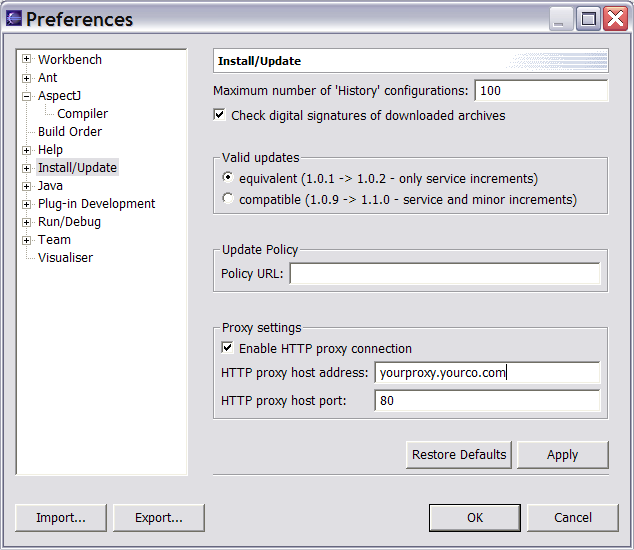
\includegraphics[width=0.80\textwidth]{./images/proxy.png}
	\caption{Setting up your proxy server}
	\label{fig:proxy}
\end{figure*}

\subsubsection{Install via Update Manager} 
Create an update site bookmark for the \cjdt ~update site, and start the install procedure.
% Ob man das brauch? \label{sec:In Eclipse 3.0}
From the help menu, select \markedtext{Software Updates} $\rightarrow$ \markedtext{Find and Install}. Select \markedtext{Search for new features to install} and click \markedtext{Next}.
Click \markedtext{Add Update Site} and enter the name \markedtext{\caesarj ~update site} and the folowing URL:  
\begin{center}
\href{http://cage.st.informatik.tu-darmstadt.de/caesar/updatesite/0.3.1}{http://cage.st.informatik.tu-darmstadt.de/caesar/updatesite/0.3.1}
\end{center}
Click \markedtext{OK}.
Fully expand the appearing \cjdt ~update site node and select \markedtext{\caesarj}. Click
\markedtext{Next}. Select \markedtext{org.caesarj.feature} as shown in figure \ref{fig:installpage30} and click \markedtext{Next}.\\

\begin{figure*}[htbp]
	\centering
		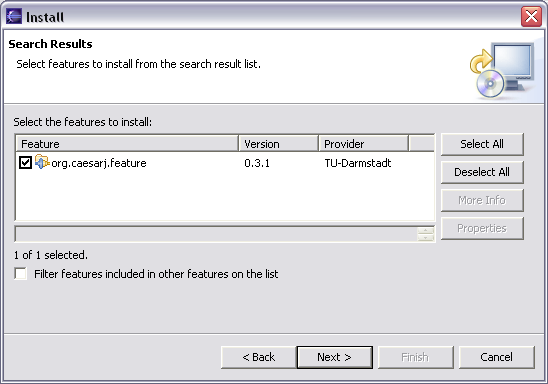
\includegraphics[width=0.85\textwidth]{./images/install_page_3_0.png}
	\caption{Selection of the \caesarj -plugin}
	\label{fig:installpage30}
\end{figure*}

Accept the \markedtext{license agreement} and proceed to the installation.

\subsection{Updating an Existing Installation}
Proceed as for a clean install, except that the \cjdt ~update site bookmark should already
exist. All you need to do, is to expand bookmark and go on. If the version you have
installed is the same as the version on the update site (or more recent even),
then you will not be presented with any install options.

\subsection{Is Everything OK?} 
Restart the Eclipse workbench. Try to open a new perspective by clicking \markedtext{Window} $\rightarrow$ \markedtext{Open Perspective}. Pick \markedtext{other} and select \markedtext{CaesarJ Perspective} in the upcoming list.
When the perspective opens successfully, the installation of your \cjdt ~works fine.
%\begin{figure}[htbp]
%	\centering
%		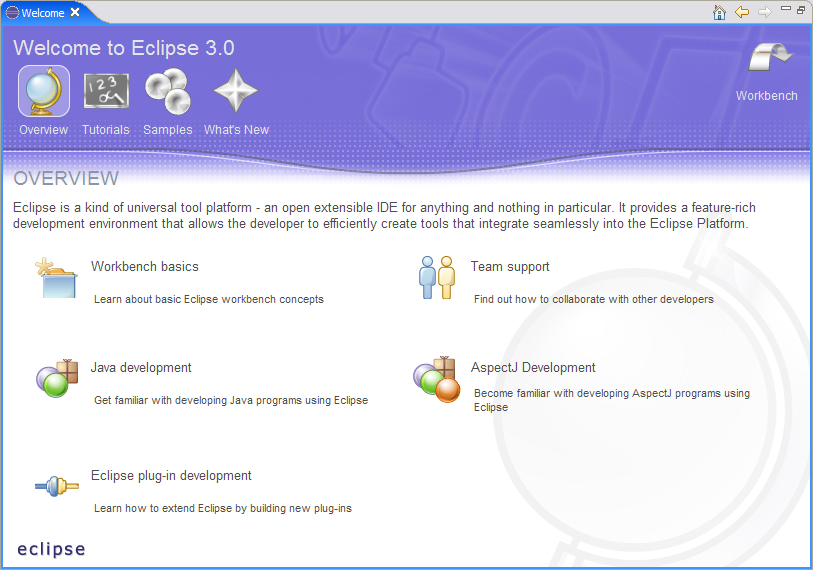
\includegraphics[width=0.95\textwidth]{./images/welcome_3_0.png}
%	\label{fig:welcome_3_0}
%\end{figure}
